\subsection{Synchronisatieprimitieven voor threads in Solaris}

Naast de gelijktijdigheid mechanismen van UNIX SVR4 ondersteunt Solaris ook:
\begin{itemize}
\item Grendels voor wederzijdse uitsluiting (mutex)
\item Semaforen
\item Grendels voor meerdere lezers en één schrijver
\item Conditievariabelen
\end{itemize}

Hieronder ziet u hoe de mechanismen eruit zien:

\begin{figure}[htp]
    \centering
            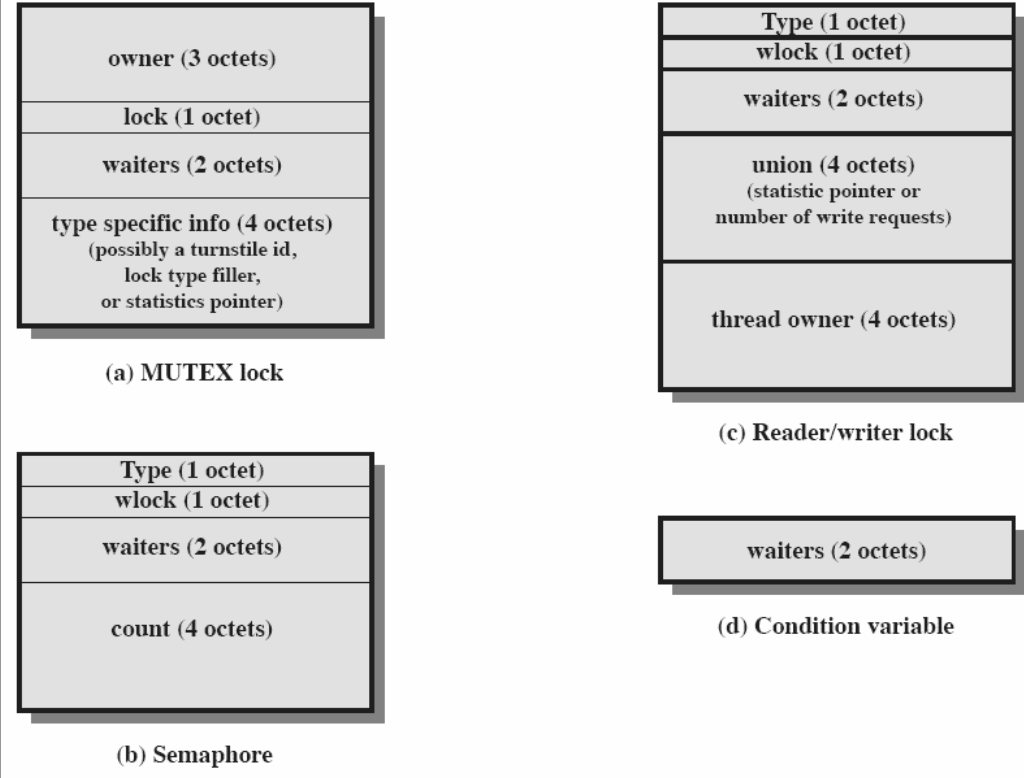
\includegraphics[width=4in]{img/mechanismen}
        \caption{Mechanismen voor synchronisatie }
    \label{fig:Mechanismen voor synchronisatie}
\end{figure}

\subsubsection{Grendel voor wederzijdse uitsluiting (MUTEX lock)}

Een mutex wordt gebruikt om zeker te zijn dat enkel 1 thread toegang heeft tot de mutex-beveiligde bron. De thread dat de mutex blokkeert moet de mutex ook deblokkeren.

\subsubsection{Semaforen}

Solaris gebruikt klassieke tellende semaforen.

\subsubsection{Lezers/schrijversgrendel}

Deze grendels laat toe meerdere threads te gelijkertijd lezers toegang te hebben tot het object dat het beveiligd. Zelfde voor schrijven, enkel 1 thread wordt tegelijkertijd toegelaten bij het schrijven en blokkeert alle lezers.

\subsubsection{Conditievariabelen}

Een conditievariabele wordt gebruikt om te wachten tot een bepaalde conditie wordt voldaan. Conditievariabelen moeten gebruikt worden in combinatie met een mutex lock.